\chapter{Introduction}
\label{sec:intro}

% \eat{
Graphs are a ubiquitous model to represent objects and their complex relations, including protein interaction and genomic graphs in biology,
chemical compound structures in chemistry, food webs and microbial taxa communities in ecology, call graphs in program flow analysis,
social networks in social science, Web graphs, as well as XML documents in e-commerce, government and medical records \cite{SH12}.
Efficient mining of hidden patterns play an important role in developing data-driven methodologies for analyzing the graphs
resulting from such datasets.

Research on graph mining has emerged as one of the hottest topics in recent years due to its wide applications in a variety of fields including
drug discovery \cite{KK01,NK05,YH02}, molecular activity prediction \cite{JYW10,TCG09},
predicting disease susceptibility from gene expression data \cite{RHS13,DI11}, software bug localization \cite{CLZWY09},
clustering and classification of graphs \cite{DKWK05,YCHY08}, anomaly detection \cite{ATK15}, and graph anonymization \cite{LAW11}.
Several variants of graph pattern mining have been proposed,
such as frequent subgraphs \cite{YH02,EASK14}, approximate subgraphs \cite{KYW10}, closed and maximal frequent subgraphs \cite{HWPY04,YH03},
discriminant and statistically significant subgraphs \cite{TCG09,RS09,YCHY08}, representative subgraphs \cite{CHSBZ08,ZYL09}, etc. --- their scalable algorithms
were implemented; besides they were extensively surveyed and compared, e.g., in \cite{HCXY07,WMFP05,AW10,KR17}.
%
\begin{figure}[t!]
\centering
\includegraphics[scale=0.32]{images/taxol}
\vspace{-2mm}
\caption{\scriptsize Correlation between {\sf CCCH} and {\sf O} in {\sf Taxol}, an anti-cancer drug. {\sf CCCH} and {\sf O}
occur closely for several times, but they are connected in different ways.}
\label{fig:taxol}
\vspace{-6mm}
\end{figure}
%


In spite of tremendous progress being made in the area of graph pattern mining, surprisingly the problem of exploring correlations between subgraphs
in a single, large graph has not been investigated in the past. In particular, we define a pair of subgraphs as correlated if
they co-occur frequently in proximity within a single graph. Correlated subgraphs are different from frequent subgraphs due to
the flexibility in which the constituent subgraphs can be connected within different instances of a correlated pattern. In Figure~\ref{fig:taxol},
we highlight three regions inside the structure of the chemical compound {\sf Taxol}, an anti-cancer drug, where {\sf CCCH} and {\sf O} occur closely,
albeit they are connected in different ways in all three instances. For simplicity, we do not consider the edge types (i.e., single- vs. double-bond)
in this example. This figure illustrates that while {\sf CCCH} and {\sf O} form a correlated subgraph pair, the individual instances, e.g., {\sf HCC(-O)C}
may not be frequent; and hence, the existing frequent subgraph mining techniques cannot be directly applied to discover such corrected patterns.


The problem of detecting correlated subgraphs from a single, large graph arises in many real-world scenarios, including biological,
social, chemical, and ecological networks, such as the ones described next.


\spara{$\bullet$ Co-operative functions in biological networks.} In the genome graph of an individual, a node represents a gene,
and each edge denotes the interaction between two genes. In practice, there are some combinations of dominant genes that
occur frequently, and they are more likely to express critical phenotypes of the individual.
Past studies have shown that some pairs of dominant gene combinations co-occur with each other in each individual,
and such co-occurring patterns reflect the joint functionality that are needed for co-operative biological functions such as chemical bonds
and binding sites \cite{LFSW14}. Based on pairs of correlated genes, we can predict co-operative biological functions of an
individual. Besides, the absence of such correlations could indicate anomalies and diseases.
Analogously, in a protein interaction (PPI) network, correlated frequent subgraphs represent recurring functional units,
identification of which could assist in predicting new protein functionalities.

\spara{$\bullet$ Co-occurrence patterns in ecological networks.}
Co-occurrence patterns are used in ecology to explore interactions between organisms
and environmental effects on co-existence within biological communities \cite{WHH14}.
Exploration of inter-taxa relationships can help identify potential biotic interactions, habitat affinities, and shared physoilogies,
that could guide more focused studies and experiments. For example, Barberan et al. \cite{BBCF12} analyzed
over 160\,000 bacterial and archaeal 16S rRNA gene sequences from 151 soil samples, collected
from a wide variety of ecosystem types, in order to demonstrate the utility of network
analyses and for evaluating whether soil microorganisms tend to co-occur more
than expected by chance, and how these
ecological categories shape network structure of inter-taxa and extra-taxa relationships.
These tasks can be achieved by mining correlated subgraphs in a single large graph
representing the soil microbial community.

\spara{Challenges.}
The problem that we study is a non-trivial one.
%
\squishlist
\item Detecting correlated subgraphs is more difficult
than the frequent subgraphs mining problem, which already has an exponential search space, that is, a graph with $m$ edges
can have $2^m$ subgraphs. For correlated subgraphs mining, the search space is doubly-exponential, because
one needs to compute the correlation between every pair of subgraphs.
\item Additionally, unlike frequent subgraphs mining,
correlated subgraphs mining is neither downward-closure, nor upward-closure (we shall demonstrate this formally
in Section~\ref{sec:problem}), thereby making it difficult to directly apply apriori-based pruning techniques.
\item Last, but not least, only finding the frequent subgraphs is not sufficient for our problem.
Instead, we require to enumerate all instances of those frequent subgraphs for computing the correlation
between pairs. This makes our problem more challenging both from computation and memory perspective.
\squishend

%We next describe why state-of-the-art techniques cannot be trivially adapted to find correlated subgraphs
%in a single, large graph.
%
%\spara{$\bullet$ Difficulties with Frequent Subgraphs Enumeration.}
%One can apply state-of-the-art frequent subgraphs mining techniques over a single graph (e.g., {\sf GRAMI} \cite{EASK14})
%to first identify all frequent subgraphs, compute correlations between every pair, and then report the
%highly correlated ones. However, this approach has several limitations.
%{\bf (1)} Many existing frequent subgraphs mining algorithms including {\sf GRAMI}
%report only the frequent subgraphs, and not their instances in the large graph.
%Thus, we separately need to enumerate all their instances using a subgraph matching algorithm
%(e.g., {\sf VF2} \cite{CFSV04}, $\textsf{Turbo}_\textsf{ISO}$ \cite{HLL13}, $\textsf{Dual}_\textsf{ISO}$ \cite{SJKFMR14}),
%which is necessary for correlation computation, but is expensive over large graphs (Figure XX).
%{\bf (2)} We are often interested in finding only the top-$k$ correlated pairs. However, the aforementioned
%frequent subgraphs mining and enumeration approach will compute correlations across every frequent subgraphs,
%which is expensive and mostly redundant. This brings the following critical question: {\em Can we mine the (top-$k$) correlated
%subgraphs in one single step}, as opposed to the aforementioned two-step frequent subgraphs mining and enumeration approach?
%The answer to this question, as we shall demonstrate in Section~\ref{sec:algorithms}, is affirmative.
%
%\begin{figure}[t!]
%\vspace{-2mm}
%\centering
%\subfigure[] {
%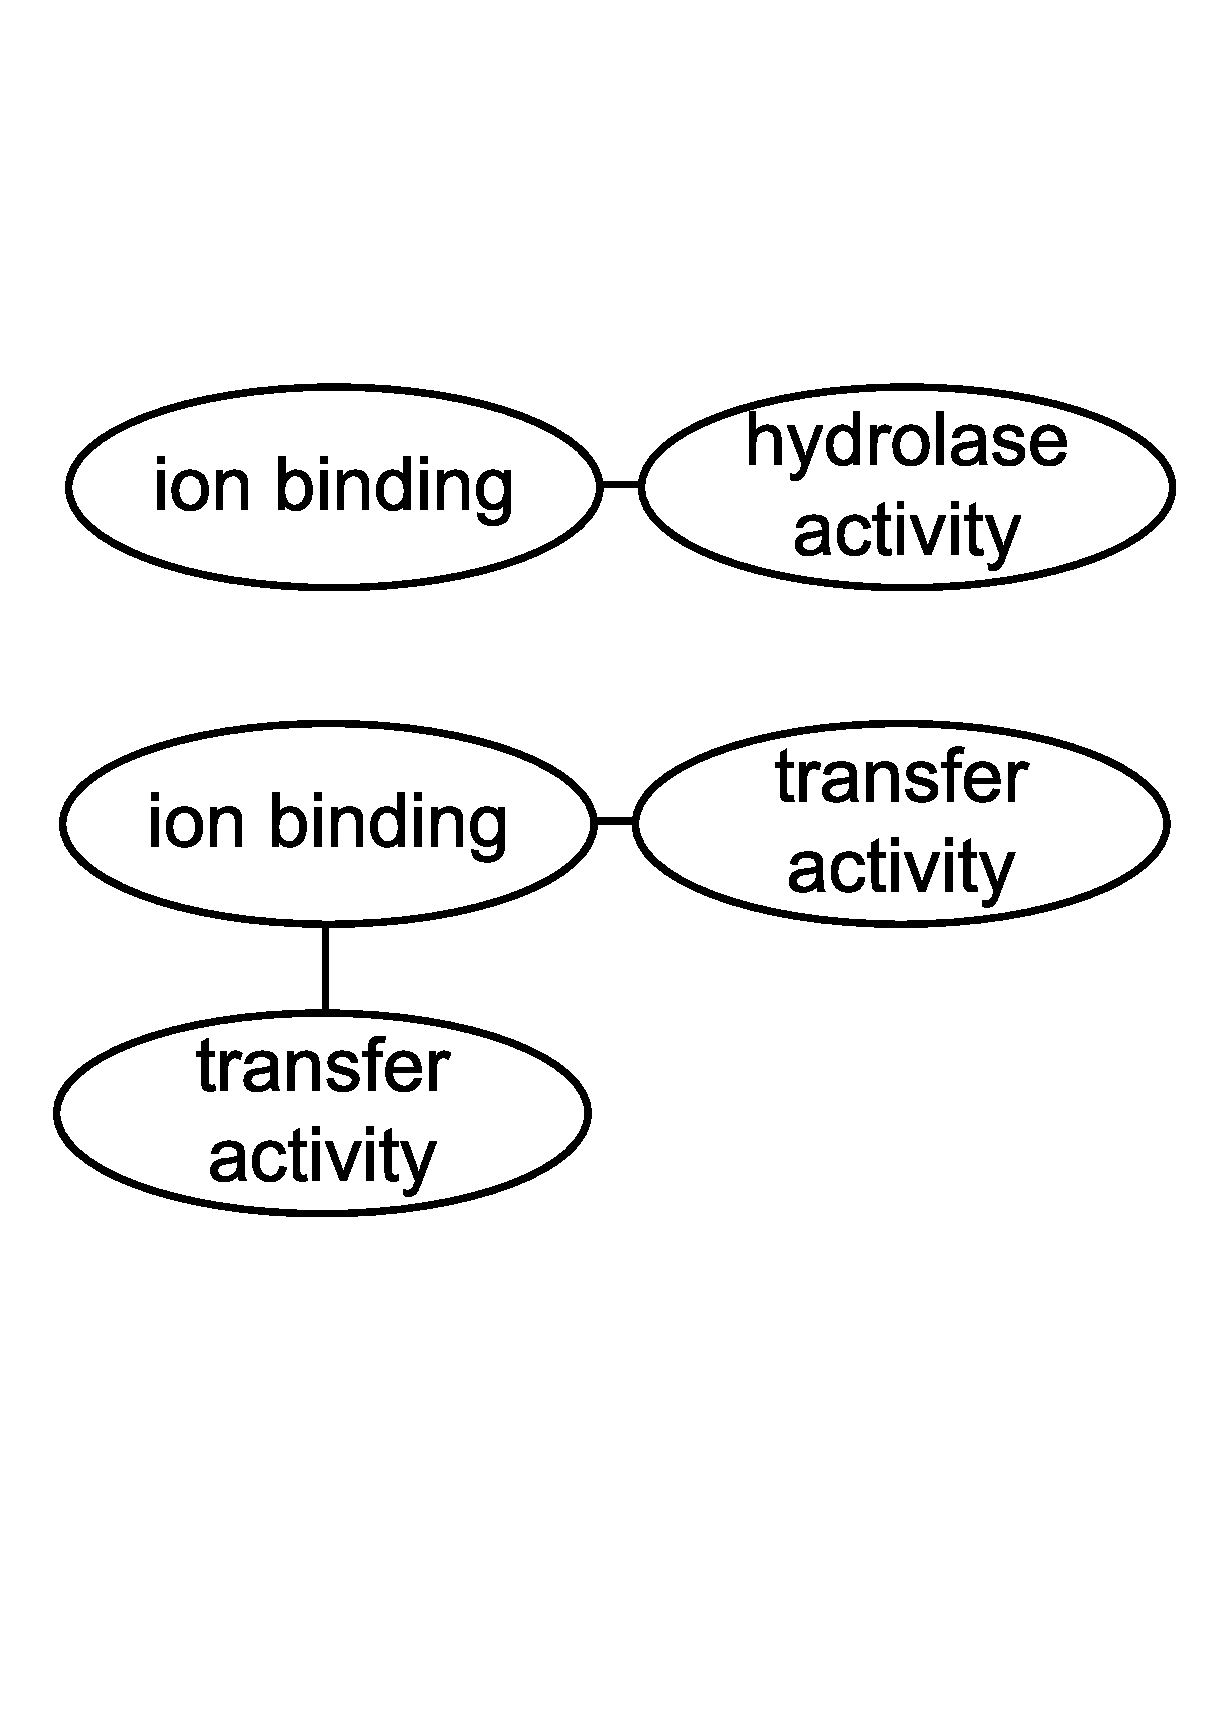
\includegraphics[scale=0.17]{images/yeast1}
%\label{fig:yeast1}
%}
%\subfigure[]  {
%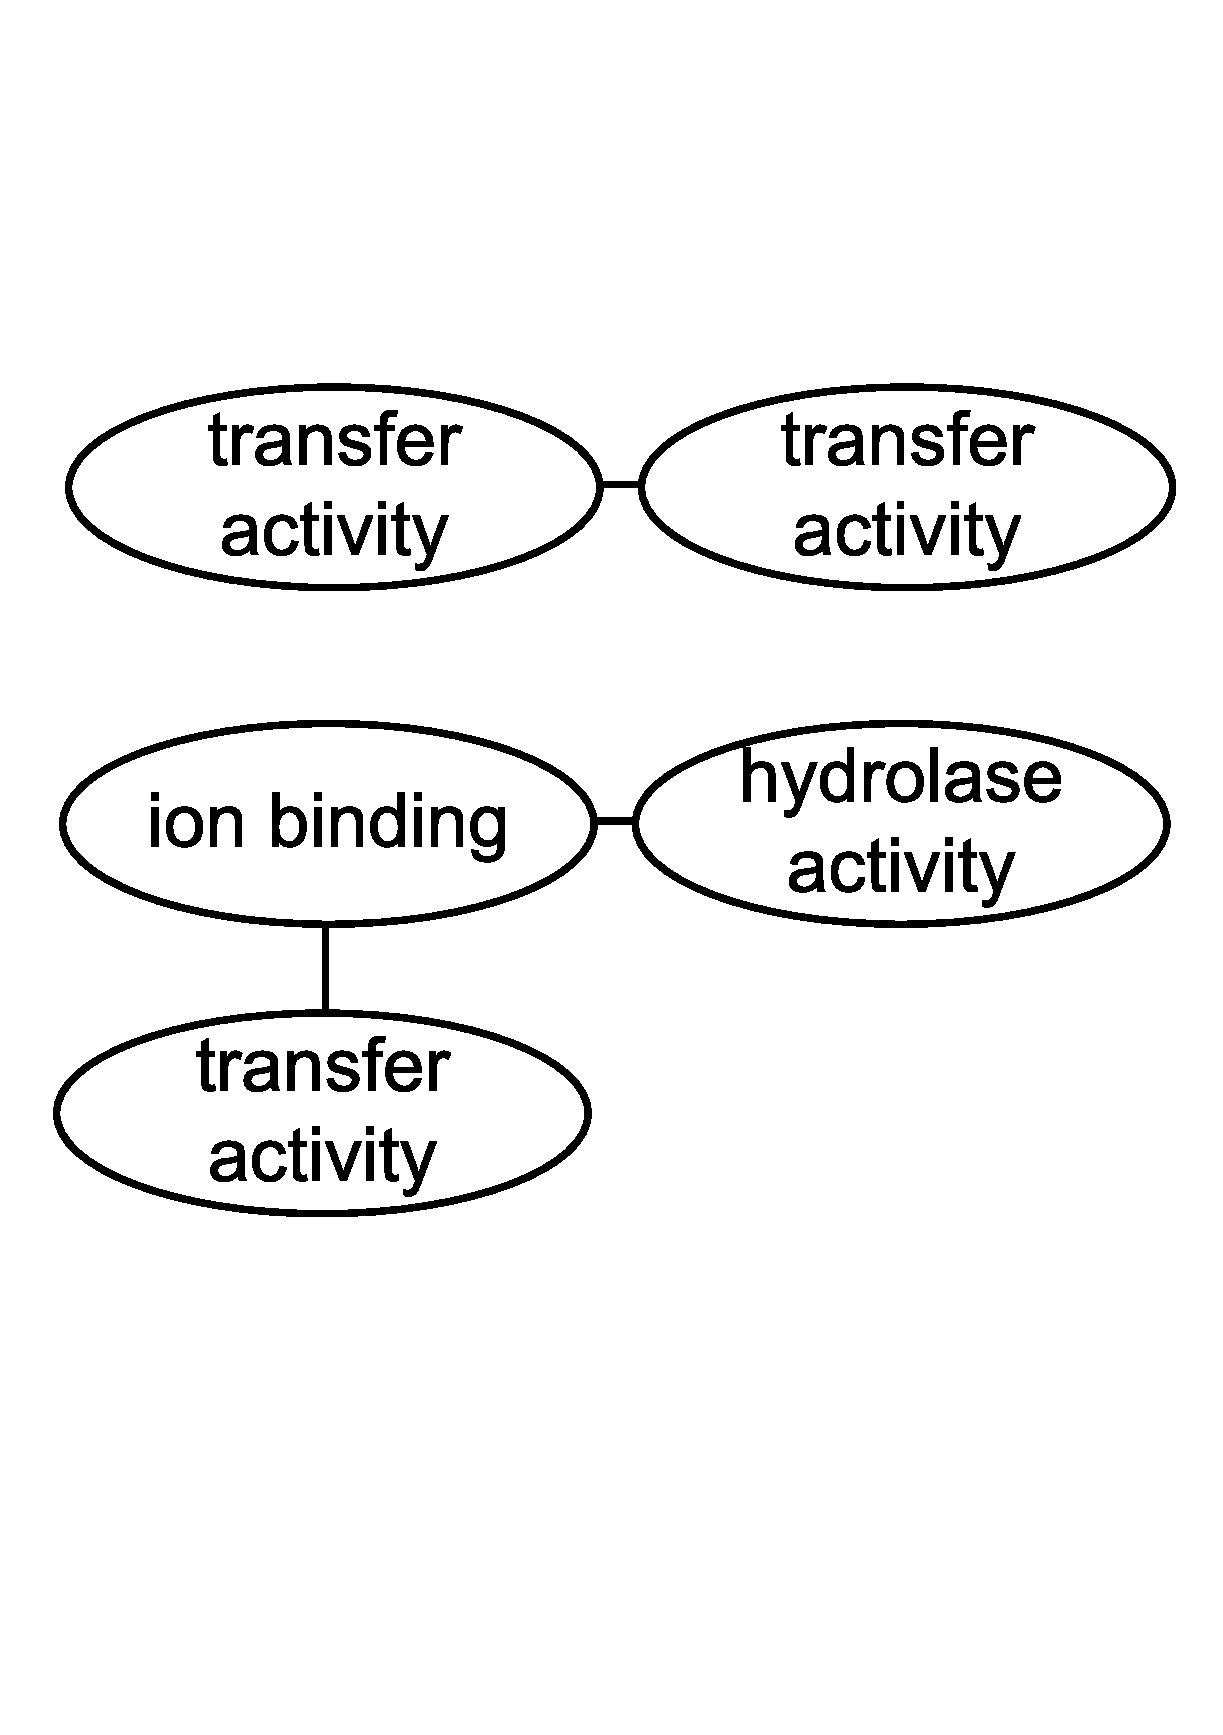
\includegraphics[scale=0.17]{images/yeast2}
%\label{fig:yeast2}
%}
%\subfigure[]  {
%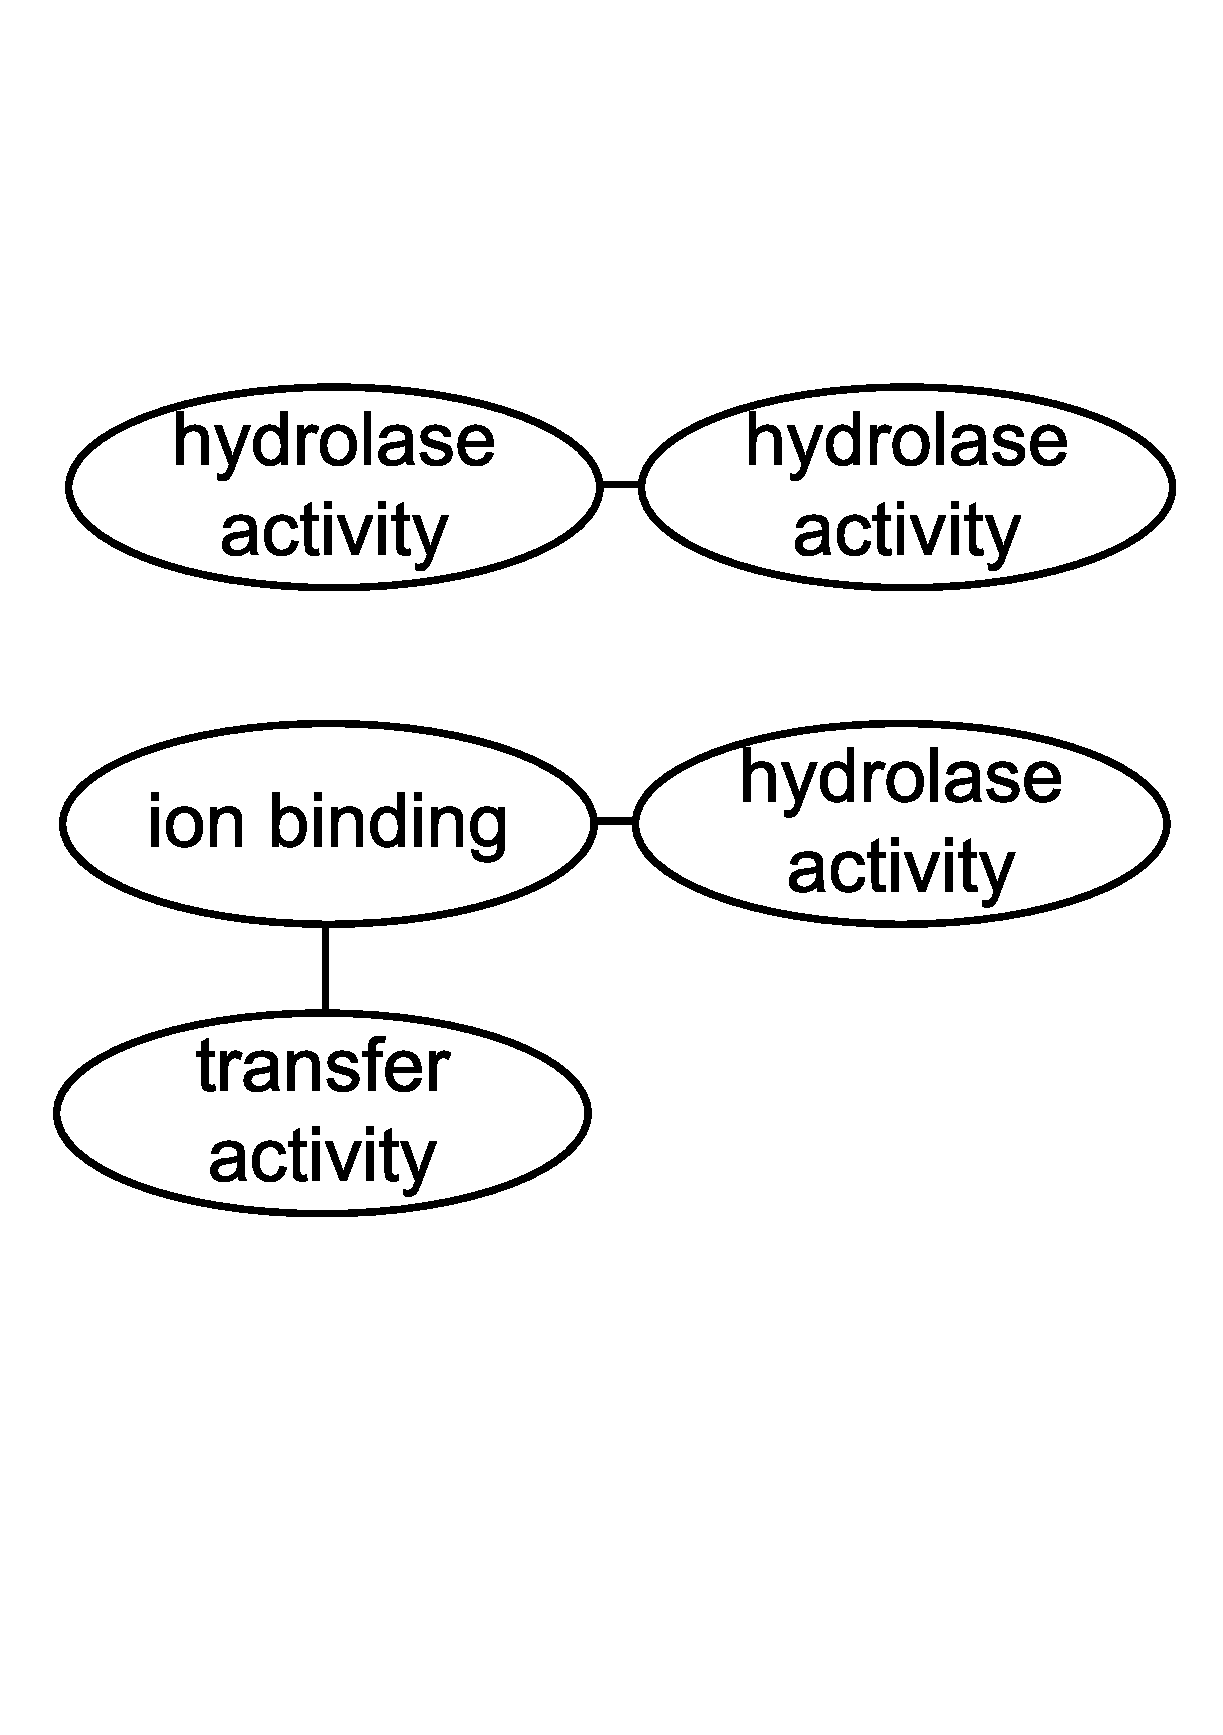
\includegraphics[scale=0.17]{images/yeast3}
%\label{fig:yeast3}
%}
%\vspace{-2mm}
%\caption{\scriptsize Correlated subgraphs discovered in the {\em Yeast} protein dataset. Nodes are annotated with protein functions (node labels).}
%\label{fig:yeast}
%\vspace{-6mm}
%\end{figure}


%\spara{$\bullet$ Difficulties with Proximity Patterns.} Recently, various approximate-frequent-subgraphs mining techniques have been
%proposed, e.g., proximity patterns \cite{KYW10} that relax the rigid structure constraint of frequent subgraphs. In stead, they identify
%a group of node labels that co-occur frequently in the neighborhood. However, such proximity patterns are often unable to capture
%the semantics of our novel correlated subgraphs. As an example, in Figure~\ref{fig:yeast},
%we present three correlated patterns identified from
%the {\em Yeast} (Saccharomyces cerevisiae) protein dataset \cite{}, where protein functions are used as node labels. These
%correlated patterns indicate that {\em transferase} and {\em hydrolase} activities are associated with {\em ion} binding,
%which is due to the fact that {\em transferase} and {\em hydrolase} undergo motions upon ligand ({\em ion}) binding
%to achieve their functions \cite{KAOK08}. However, {\em transferase} and {\em hydrolase} catalyze different chemical
%reactions and express different dynamic responses upon ligand ({\em ion}) binding. It means that {\em hydrolase} and {\em transferase}
%activities are usually not connected with each other directly and they usually connect to {\em ion} binding \cite{KKO09}.
%This is indeed reflected in our discovered correlated patterns, because there is no direct edge between {\em hydrolase} and {\em transferase}.
%On the other hand, the proximity pattern mining algorithm \cite{KYW10} reports
%$\langle${\em hydrolase}, {\em transferase}, {\em ion binding}$\rangle$ as one
%proximity pattern, thus it is unable to capture the fact that {\em hydrolase} and {\em transferase}
%activities are not connected with each other directly.

\spara{Our contributions and roadmap.}
To this end, we design a single-step, best-first exploration algorithm to detect correlated subgraphs,
coupled with efficient top-$k$ pruning and various optimization techniques.
The main contributions of this paper are as follows:
\squishlist
\item
\item
\item
\item We empirically demonstrate effectiveness and efficiency of our methods on real-life graphs,
while also detailing three concrete case studies (Section \ref{sec:experiments}).
\squishend
% }

